% 2014 Este modelo foi desenvolvido pelo grupo PET Engenharia Mecânica (pet-em@dem.feis.unesp.br) baseado no modelo de Curriculum Vitae desenvolvido pelos autores citados abaixo:
% 2002 Matthew Boedicker <mboedick@mboedick.org> (original author) http://mboedick.org
% 2003-2007 David J. Grant <davidgrant-at-gmail.com> http://www.davidgrant.ca
% 2008 Nathaniel Johnston <nathaniel@nathanieljohnston.com> http://www.nathanieljohnston.com


\documentclass[letterpaper,11pt]{article}
\usepackage[utf8]{inputenc} 
\usepackage[T1]{fontenc}
\usepackage[portuges,brazil]{babel}    			% hifenação em português
\newlength{\outerbordwidth}
\pagestyle{empty}
\raggedbottom
\raggedright
\usepackage[svgnames]{xcolor}
\usepackage{framed}
\usepackage{tocloft}
\usepackage{graphicx}
\usepackage{multicol}
\usepackage{amsmath,amssymb}
\usepackage{epstopdf}

%-----------------------------------------------------------
%Altere estes valores para modificar a aparência das caixas de textos

\setlength{\outerbordwidth}{3pt}  % Tamanho da borda dos títulos
\definecolor{shadecolor}{gray}{0.75}  % Define a cor cinza através da escala de cinza, para o vlaor 0 temos preto e 1 temos branco
\definecolor{shadecolorB}{gray}{0.95}  % Cor de fundo da caixa de títulos 


%-----------------------------------------------------------
%Informações das margens

\setlength{\evensidemargin}{-0.25in}
\setlength{\headheight}{0in}
\setlength{\headsep}{0in}
\setlength{\oddsidemargin}{-0.25in}
\setlength{\paperheight}{11in}
\setlength{\paperwidth}{8.5in}
\setlength{\tabcolsep}{0in}
\setlength{\textheight}{9.5in}
\setlength{\textwidth}{7in}
\setlength{\topmargin}{-0.3in}
\setlength{\topskip}{0in}
\setlength{\voffset}{0.1in}


%-----------------------------------------------------------
%Comandos customizados
\newcommand{\resitem}[1]{\item #1 \vspace{-2pt}}
\newcommand{\resheading}[1]{\vspace{8pt}
  \parbox{\textwidth}{\setlength{\FrameSep}{\outerbordwidth}
    \begin{shaded}
\setlength{\fboxsep}{0pt}\framebox[\textwidth][l]{\setlength{\fboxsep}{4pt}\fcolorbox{shadecolorB}{shadecolorB}{\textbf{\sffamily{\mbox{~}\makebox[6.762in][l]{\large #1} \vphantom{p\^{E}}}}}}
    \end{shaded}
  }\vspace{-5pt}
}
\newcommand{\ressubheading}[4]{
\begin{tabular*}{6.5in}{l@{\cftdotfill{\cftsecdotsep}\extracolsep{\fill}}r}
		\textbf{#1} & #2 \\
		\textit{#3} & \textit{#4} \\
\end{tabular*}\vspace{-6pt}}
%-----------------------------------------------------------


%--------------------------------------
%comandos para aumentar chaves e parênteses
\newcommand{\PR}[1]{\ensuremath{\left[#1\right]}}
\newcommand{\PC}[1]{\ensuremath{\left(#1\right)}}
\newcommand{\chav}[1]{\ensuremath{\left\{#1\right\}}}
%--------------------------------------

\begin{document}
\begin{center}
\textbf{\Large Experimento 1 e 2 - Modelo canônico Relatório onepage}
\end{center}
\begin{tabular*}{7in}{l@{\extracolsep{\fill}}r}
 & \\
 Fulano de tal & 11050000 \\
 Ciclano de tal & 11050001\\
  & Ilha Solteira, \today\\
\end{tabular*}
\\


%%%%%%%%%%%%%%%%%%%%%%%%%%%%%%
\resheading{Objetivo}
%%%%%%%%%%%%%%%%%%%%%%%%%%%%%%
Aqui ficará o objetivo do experimento, sempre com informações sucintas.

%%%%%%%%%%%%%%%%%%%%%%%%%%%%%%
\resheading{Introdução}
%%%%%%%%%%%%%%%%%%%%%%%%%%%%%%
Em um relatório onepage a introdução deve ser extremamente direta. Só coloque as equações que irá utilizar e nada de explicações profundas sobre a teoria.

Segundo a lei do resfriamento de Newton:
\begin{equation}
q'' = h(T_{s} - T_{\infty})
\label{eqi}
\end{equation}


\resheading{Metodologia}
\textbf{Experimento 1:} 
Dê as informações gerais importantes do processo empregado no experimento.
\\
\
\\
\textbf{Experimento 2:}
Note que separamos em diferentes experimentos, é uma maneira organizada de detalhamento.

%%%%%%%%%%%%%%%%%%%%%%%%%%%%%%
\resheading{Resultados}
%%%%%%%%%%%%%%%%%%%%%%%%%%%%%%
Aqui apresente os dados utilizados por tabelas de referência, informações fundamentais para os cálculos. Os resultados obtidos no experimento devem estar preferencialmente contidos em tabelas e gráficos. 
\\
\
\\
\textbf{Experimento 1:}
Neste experimento, os resultados foram apresentados na tabela \ref{tab1}.
\\

\begin{table}[ht]
	\centering
	\caption{Resultados do experimento 1.}
\begin{tabular}{c c c}
\hline 
\hspace{0.3cm}Número de abobrinhas&\hspace{0.3cm}\textbf{$Temperatura [^{\circ}\mathrm{C}]$}&\hspace{0.3cm}\textbf{$D[cm]$}\\ 
\hline 
0 & 84 & - \\ 
\hline 
670 & 80 & 21,8\\ 
\hline 
1450 & 76 & 18,7\\ 
\hline 
2280 & 72 & 17,6\\ 
\hline 
3170 & 68 & 16,4\\ 
\hline 
4130 & 64 & 15,2\\ 
\hline 
\end{tabular} 
\label{tab1}
\end{table}

\newpage
\textbf{Experimento 2:} 
O resultado obtido no experimento 2 esta contido no gráfico \ref{fig:graf1}.

\begin{figure}[!htp]
\caption{Resultado do experimento 2}
\begin{center}
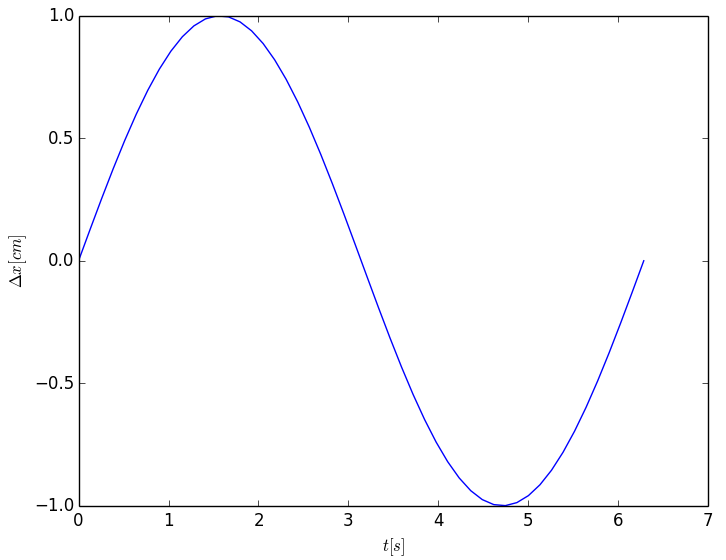
\includegraphics[scale=0.5]{graf.png} 
\end{center}
\begin{center}
\scriptsize{Fonte: Própria}
\end{center}
\label{fig:graf1}
\end{figure}
%%%%%%%%%%%%%%%%%%%%%%%%%%%%%%
\resheading{Conclusões}
%%%%%%%%%%%%%%%%%%%%%%%%%%%%%%
Apresente as conclusões baseadas nos resultados do item anterior.
\end{document}